\begin{center}
  \resizebox{0.9\linewidth}{!}{
    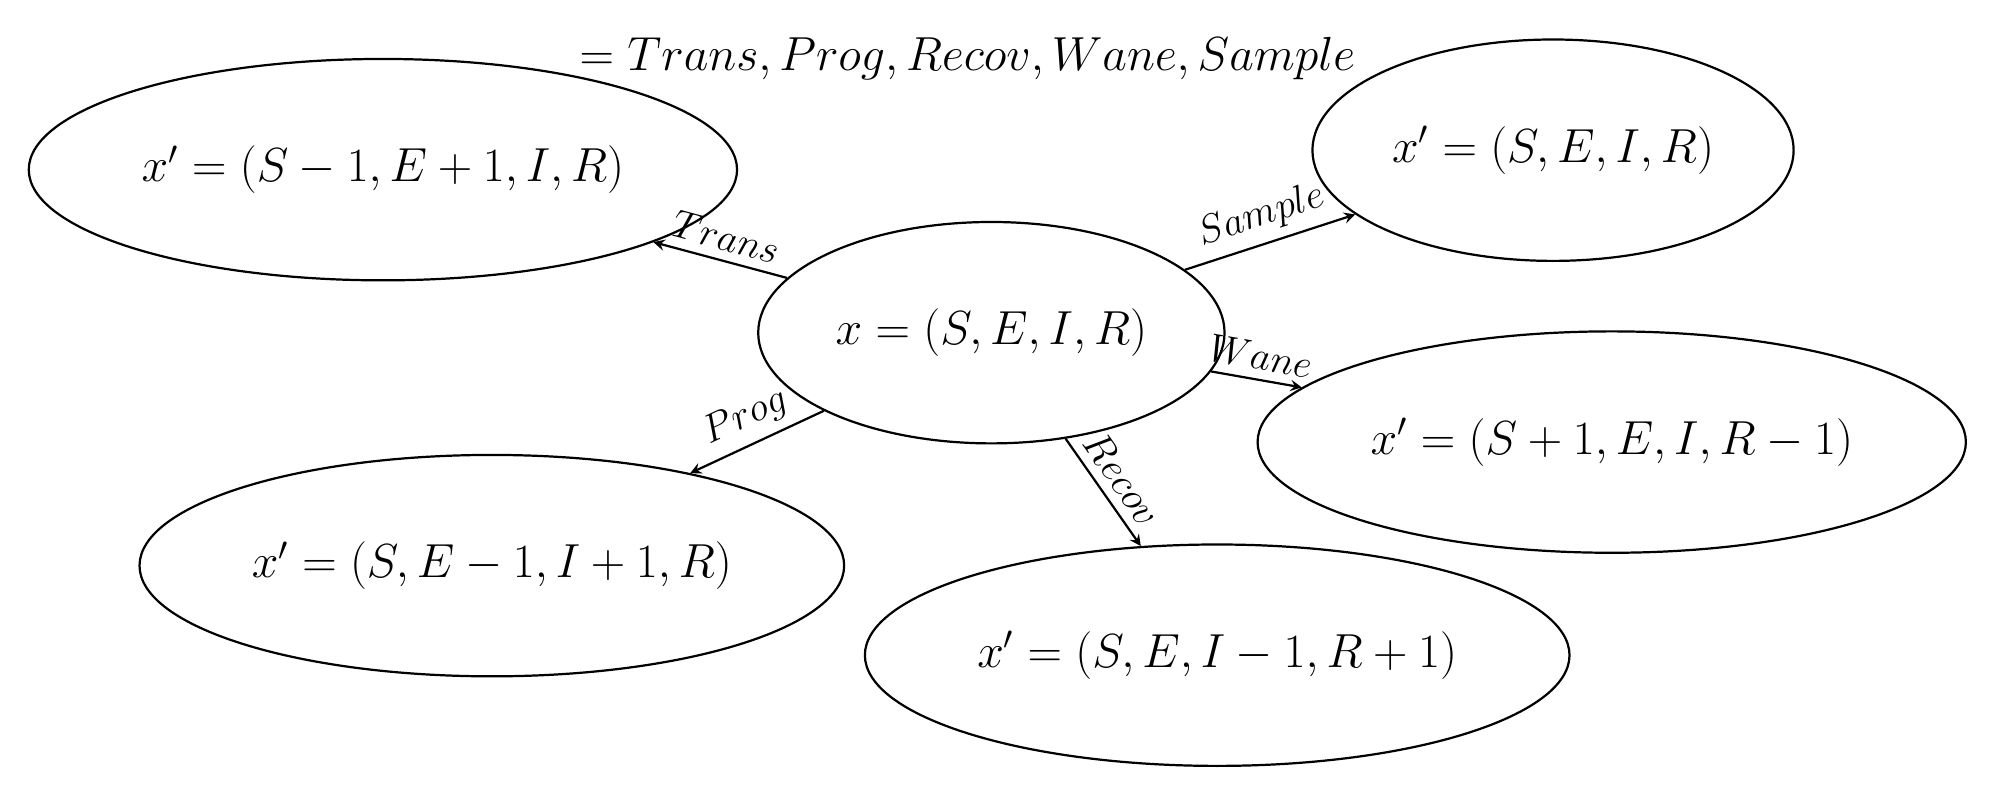
\begin{tikzpicture}[scale=1]
      \usetikzlibrary{shapes,arrows,positioning}
      \tikzstyle{coordinate}=[inner sep=0pt,outer sep=0pt]
      \tikzstyle{state}=[shape=ellipse, color=black, draw, font=\LARGE, fill=white, thick, minimum height=8em]
      \tikzstyle{trans}=[color=black, font=\Large, thick, >=stealth]
      \node[state] (base) at (0,0) {$x=(S,E,I,R)$};
      \node[state] (trans) at (165:8) {$x'=(S-1,E+1,I,R)$};
      \node[state] (prog) at (205:7) {$x'=(S,E-1,I+1,R)$};
      \node[state] (recov) at (305:5) {$x'=(S,E,I-1,R+1)$};
      \node[state] (wane) at (350:8) {$x'=(S+1,E,I,R-1)$};
      \node[state] (sample) at (18:7.5) {$x'=(S,E,I,R)$};
      \draw[trans,->] (base) -- (trans) node[midway,above,sloped] {$\lab{Trans}$};
      \draw[trans,->] (base) -- (prog) node[midway,above,sloped] {$\lab{Prog}$};
      \draw[trans,->] (base) -- (recov) node[midway,above,sloped] {$\lab{Recov}$};
      \draw[trans,->] (base) -- (wane) node[midway,above,sloped] {$\lab{Wane}$};
      \draw[trans,->] (base) -- (sample) node[midway,above,sloped] {$\lab{Sample}$};
      \node[font=\LARGE] (U) at (95:3.5) {$\Jumps=\Set{\lab{Trans},\lab{Prog},\lab{Recov},\lab{Wane},\lab{Sample}}$};
    \end{tikzpicture}
  }
\end{center}
\caption{
  Markov state transition diagram for the SEIRS model depicted in \cref{fig:example_models}A.
  The state, $x$, is characterized by four numbers, $S$, $E$, $I$, and $R$.
  From a given state $x$, there are five possible kinds of jumps $x\mapsto{x'}$.
  Accordingly, the set, $\Jumps$, of jump marks has five elements.
  Each of these is of a different type:
  $\lab{Trans}$ (transmission) is of birth type,
  $\lab{Prog}$ (progression) is of migration type,
  $\lab{Recov}$ (recovery) is of death type,
  $\lab{Sample}$ (sampling) is of sample type,
  and $\lab{Wane}$ (loss or waning of immunity) is of neutral type.
  See \cref{sec:event_types} for a description of these jump types.
  Note that, in this formulation, when a sampling event occurs, the state does not change.
  \label{fig:markov_state}
}
